\documentclass{book}

\usepackage{libertine}

\usepackage{graphicx}
\graphicspath{ {images/} }
\usepackage{listings}
\usepackage{color}
\usepackage{tikz}
\definecolor{mygreen}{rgb}{0,0.6,0}
\definecolor{gray}{rgb}{0.4,0.4,0.4}
\definecolor{darkblue}{rgb}{0.0,0.0,0.6}
\definecolor{cyan}{rgb}{0.0,0.6,0.6}
\usepackage[top=3cm, bottom=2cm, outer=3cm, inner=2.1cm, headsep=14pt]{geometry}
\usepackage[framemethod=tikz]{mdframed}
\definecolor{boxcolor}{rgb}{0.122, 0.435, 0.698}
\usepackage{hyperref}

\newmdenv[innerlinewidth=0.5pt, roundcorner=4pt,linecolor=boxcolor,innerleftmargin=6pt,
innerrightmargin=6pt,innertopmargin=6pt,innerbottommargin=6pt]{coloredbox}
\newcommand{\shrug}[1][]{%
	\begin{tikzpicture}[baseline,x=0.8\ht\strutbox,y=0.8\ht\strutbox,line width=0.125ex,#1]
	\def\arm{(-2.5,0.95) to (-2,0.95) (-1.9,1) to (-1.5,0) (-1.35,0) to (-0.8,0)};
	\draw \arm;
	\draw[xscale=-1] \arm;
	\def\headpart{(0.6,0) arc[start angle=-40, end angle=40,x radius=0.6,y radius=0.8]};
	\draw \headpart;
	\draw[xscale=-1] \headpart;
	\def\eye{(-0.075,0.15) .. controls (0.02,0) .. (0.075,-0.15)};
	\draw[shift={(-0.3,0.8)}] \eye;
	\draw[shift={(0,0.85)}] \eye;
	% draw mouth
	\draw (-0.1,0.2) to [out=15,in=-100] (0.4,0.95); 
	\end{tikzpicture}}
\lstdefinestyle{customcs}{
	frame=single,
	basicstyle=\footnotesize\ttfamily, 
	tabsize=2, 
	extendedchars=true, 
	breaklines=true, 
	stringstyle=\color{red}\ttfamily, 
	showspaces=false, 
	showtabs=false, 
	commentstyle=\color{gray},
	morecomment=[l]{//},
	morecomment=[s]{/*}{*/},
	showstringspaces=false, 
	morekeywords={  abstract, event, new, struct,
		as, explicit, null, switch,
		base, extern, object, this,
		bool, false, operator, throw,
		break, finally, out, true,
		byte, fixed, override, try,
		case, float, params, typeof,
		catch, for, private, uint,
		char, foreach, protected, ulong,
		checked, goto, public, unchecked,
		class, if, readonly, unsafe,
		const, implicit, ref, ushort,
		continue, in, return, using,
		decimal, int, sbyte, virtual,
		default, interface, sealed, volatile,
		delegate, internal, short, void,
		do, is, sizeof, while,
		double, lock, stackalloc,
		else, long, static,
		enum, namespace, string, var},
	keywordstyle=\color{blue},
	identifierstyle=\color{cyan},
}

\lstdefinestyle{customc}{
	basicstyle=\ttfamily,
	columns=fullflexible,
	showstringspaces=false,
	commentstyle=\color{gray}\upshape,
	belowcaptionskip=1\baselineskip,
	breaklines=true,
	frame=single,
	xleftmargin=\parindent,
	language=C,
	showstringspaces=false,
	basicstyle=\footnotesize\ttfamily,
	keywordstyle=\bfseries\color{blue},
	commentstyle=\itshape\color{gray},
	identifierstyle=\color{black},
	stringstyle=\color{red},
}

\lstdefinelanguage{XML}
{
	morestring=[b]",
	morestring=[s]{>}{<},
	morecomment=[s]{<?}{?>},
	stringstyle=\color{black},
	identifierstyle=\color{darkblue},
	keywordstyle=\color{cyan},
	morekeywords={xmlns,version,type}% list your attributes here
}

\lstdefinestyle{custombash}
{
	frame=single,
	basicstyle=\footnotesize\ttfamily,
	columns=fullflexible,
	showstringspaces=false
}

\lstdefinestyle{customxml}
{
	frame=single,
	basicstyle=\footnotesize\ttfamily,
	columns=fullflexible,
	showstringspaces=false
}

\begin{document}

\author{Tyler Crandall}
\title{Advanced C\# for Low-Level Programming\\
	   \large Licensed Attribution-NonCommercial 3.0 
	   \\United States (CC BY-NC 3.0 US) \\
   	   \small https://creativecommons.org/licenses/by-nc/3.0/us/}
\date{November 2018}

\frontmatter

\maketitle
\newpage
\large Book Contributors \newline
\begin{itemize}
	\item Jamesbascle - For grammar corrections.
	\item Topping - For grammar corrections.
	\item SirJosh3917 - For correcting Chapter 4 Snippet, renamed chapFourLib to lib variable.
\end{itemize}

\newpage
\tableofcontents

\mainmatter
\chapter{Introduction}
\section{Ce dont vous avez besoin pour commencer}
Vous avez besoin de Dotnet Core et du compilateur Clang/LLVM pour suivre ce livre. Les exemples de ce livre sont prévues pour être utilisé dans un environnement Linux, bien que les connaissances acquises ici puissent être appliquées à toute autre plateforme, y compris Windows.

Vous pouvez installer Dotnet Core SDK depuis cette URL et suivre les instructions d'installation selon votre plateforme :
\newline \newline
 https://www.microsoft.com/net/download/linux
\newline \newline
Le compilateur Clang/LLVM peut être installé selon votre distribution, voici une aide au démarrage.
\newline \newline
\begin{tabular}{| c | c |}
	\hline 
	\textbf{Linux Distribution} & \textbf{Command Line or Link} \\
	\hline
	 Arch Linux & pacman -S llvm clang  \\
	 \hline
	 Ubuntu & apt.llvm.org/ \\
	 \hline
	 Debian & apt.llvm.org/ \\
	 \hline
	 Red Hat Enterprise Linux & developers.redhat.com/blog/2018/07/07/yum-install-gcc7-clang/ \\
	 \hline
	 Fedora & dnf install llvm clang \\
	 \hline
	 CentOS & Compile LLVM/Clang yourself  \shrug \\
	 \hline
	 OpenSUSE & zypper install llvm clang \\
	 \hline
	 Gentoo Linux & https://wiki.gentoo.org/wiki/Clang \\
	 \hline
	 Slackware Linux & Compile LLVM/Clang yourself  \shrug \\
	 \hline
\end{tabular}

\section{Minimum Knowledge}
Vous aurez besoin d'avoir les bases en C# et C avant de commencer ce livre, qui tentera toutefois de vous expliquer les bases du C / C++.
\chapter{Introduction au P/Invoke}

\section{Commençons}
Tout d'abord, créer un dossier 'ChapterTwo' pour le projet et créer un nouveau fichier, 'ChapTwo.c' dans le dossier 'ChapterTwo'.

Supposons que nous ayons une fonction d’addition de base dans une bibliothèque C que nous voulons appeler.

\lstinputlisting[style=customc, language=C]{codes/Chap2/Chap2Snippet1.c}

Au premier abord nous pourrions croire qu'il s'agit d'une simple opération d'addition, mais il y a quelques considérations qui doivent être observées d'abord avant d'essayer d'écrire le code d'enveloppe d'invocation de plate-forme pour la fonction ci-dessus :

\begin{enumerate}
	\item \label{itm:first} le type `int` en C peut être considéré comme long de 2 ou 4 octets ou aussi long qu'il puisse être selon l'architecture et le compilateur sur lequel la bibliothèque est compilée. Dans la norme C, int doit être capable de contenir \textbf{au moins} l'intervalle [\textminus32,767, +32,767]; ainsi, sa taille est d'au moins 16 bits.
	
	\item En raison de \ref{itm:first}, vous pouvez raisonnablement vous prémunir contre la perte de données en remplaçant C\# Int32(int) qui contient 4 octets, ou vous pouvez choisir de suivre la norme strictement en fournissant C\# Int16(short) qui contient 2 octets, même s'il peut subir des pertes de données. La meilleure approche est d'éviter d'utiliser "au moins" des entiers en C et d'utiliser des entiers de taille fixe fournis par le compilateur dans le fichier ''stdint.h'' si vous avez gardé à l'esprit l'interface de la fonction externe..
	
	\item Parfois, il faut garder à l'esprit l'endianité, bien qu'elle soit moins préoccupante dans les architecture x86\_64 la petite endianesse est la valeur par défaut.
\end{enumerate}
La meilleure approche pour écrire la fonction Addition est d'indiquer clairement la taille des entiers que vous essayez d'ajouter si possible.

\lstinputlisting[style=customc, language=C]{codes/Chap2/Chap2Snippet2.c}

\section{Compiler la Library}
Ce livre suppose que vous avez une connaissance suffisante de C, nous vous fournirons tout de même des instructions de compilation. La commande suivante suppose que vous avez nommé votre fichier de code source : ' ChapTwo.c' comme indiqué au début de ce chapitre.
\lstinputlisting[style=custombash,language=Bash]{codes/Chap2/Chap2Snippet3.sh}

Ici nous examinons et expliquons les arguments du compilateur :

\begin{enumerate}
	\item '-std=c99' spécifie que nous compilons le code source C sous le standard C99.
	\item '-shared' spécifie que nous voulons que le programme soit compilé en tant que bibliothèque partagée/dynamique.
	\item '-fPIC' spécifie que le code doit être indépendant de la position afin que la bibliothèque résultante puisse être chargée par d'autres processus et que le code soit disponible pour être exécuté n'importe où dans l'espace d'adresse du programme indépendamment de l'adresse du code.
	\item '-olibChapTwo.so' spécifie le nom de la bibliothèque de sortie. Le préfixe lib dans'libChapTwo.so' est une question de convention de nommage à suivre sous Linux bien que les compilateurs comme clang et gcc recherchent les bibliothèques basées sur le préfixe lib en utilisant l'option'-l'. 
\end{enumerate}
\newpage
\section{Configuring C\# Project}
Puisque nous sommes déjà dans le répertoire "ChapterTwo", nous pouvons lancer 'dotnet new Console'. Il y a quelques étapes que nous devons prendre pour ajouter le code C à notre projet C\#. Tout d'abord, nous devons automatiser le processus de compilation de notre fichier C et copier la bibliothèque C compilée dans le répertoire cible pour la configuration Debug, Release ou toute autre configuration..

Ouvrez le fichier 'ChapterTwo.csproj' avec votre éditeur préféré, et ajoutez ce qui suit sous '</PropertyGroup>' dans la balise '<Project>'.

\lstinputlisting[style=customxml, language=XML]{codes/Chap2/Chap2Snippet4.xml}

L'extrait ci-dessus fait peu de choses après la construction de notre projet C\# :

\begin{enumerate}
	\item Compiler le code ChapTwo.c comme une bibliothèque partagée, libChapTwo.so
	\item Copiez libChapTwo.so dans n'importe quel répertoire cible dans lequel C\# est construit.
\end{enumerate}

Il est ainsi beaucoup plus facile de modifier notre code sans avoir à exécuter de commandes supplémentaires pour qu'il prenne effet.

Votre CSProj devrait ressembler à ce qui suit :

\lstinputlisting[style=customxml, language=XML]{codes/Chap2/Chap2Snippet5.xml}
\newpage
\section{Appeler le code C en C\#}
Ouvrez Program.cs, ajoutez une nouvelle directive d'utilisation en haut de votre code source.

\lstinputlisting[style=customcs]{codes/Chap2/Chap2Snippet6.cs}

Cette ligne importe tous les services d'invocation de la plate-forme, ce qui nous permet d'interagir facilement avec notre bibliothèque C.

Ajoutez les lignes suivantes sous dans votre classe Program :

\lstinputlisting[style=customcs]{codes/Chap2/Chap2Snippet7.cs}

L'attribut DllImport déclare qu'une fonction statique définie en externe est définie dans une bibliothèque C et que CLR doit créer un stub d'Invocation de Plate-forme pour définir ladite fonction dans une bibliothèque externe.

Il est nécessaire de déclarer la fonction avec des modificateurs statiques et externes puisque c'est une fonction qui est à la fois indépendante de l'état et définie de l'extérieur.

Enfin, modifiez la ligne ''Console.WriteLine''' comme suit :

\lstinputlisting[style=customcs]{codes/Chap2/Chap2Snippet8.cs}
Et votre code source devrait ressembler à ce qui suit :

\lstinputlisting[style=customcs, language={[Sharp]C}]{codes/Chap2/Chap2Snippet9.cs}
\newpage
Enfin, votre programme est prêt à être exécuté. Tu peux le lancer :
\lstinputlisting[style=custombash,language=Bash]{codes/Chap2/Chap2Snippet10.sh}

Et nous obtenons ce qui suit :

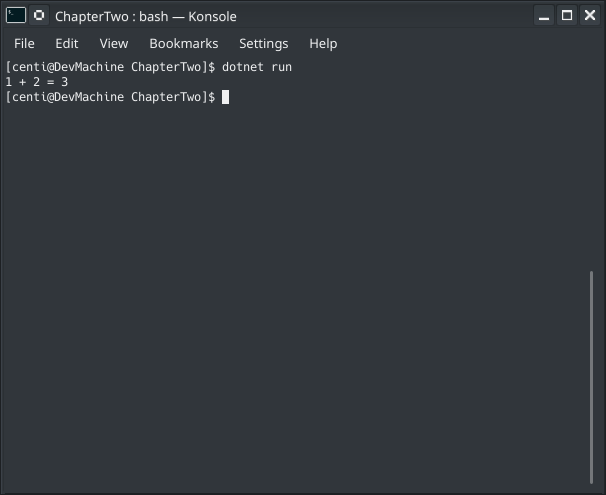
\includegraphics[width=\textwidth]{ChapTwoConsole}
Cela fonctionne comme prévu !
\newpage
\section{Some Backgrounds}
Il se passe peu de choses lorsqu'une fonction avec DllImport est appelée, si c'est la première fois que la fonction est appelée, le Runtime chargera d'abord la bibliothèque externe immédiatement, puis chargera la méthode ''Sum'' lorsque la méthode définie par P/Invoke est appelée, et enfin générera un P/Invoke pour cette fonction pour supporter l'appel à la fonction externe.

Le symbole n'est que cela, un symbole exporté par la bibliothèque C qui peut être résolu à une adresse où se trouve le code ou la variable. Vous pouvez trouver une liste de symboles en exécutant ''objdump -T libChapTwo.so'' sur votre bibliothèque et vous aurez ce qui suit :

\newline \newline
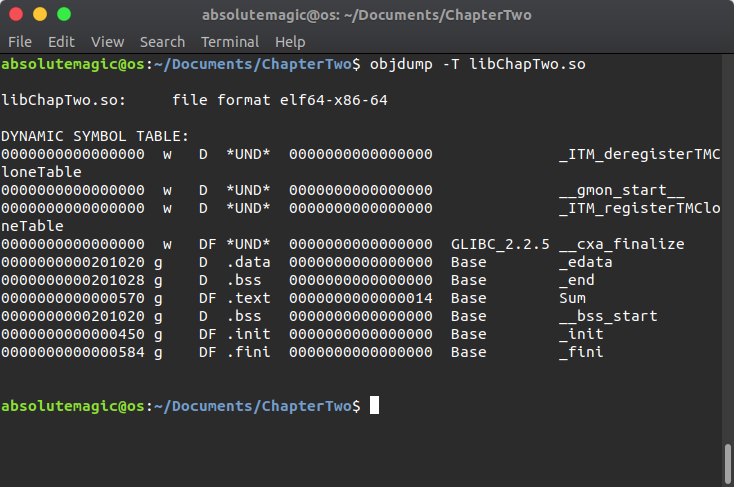
\includegraphics[width=\textwidth]{ChapTwoConsoleTwo}
\newline\newline
Vous remarquerez que le symbole Sum est affiché dans le tableau des symboles de votre bibliothèque, c'est ainsi que la CLR recherche une fonction par nom d'entrée.
\include{./TeX_files/chapter03}
\chapter{The History On Delegate Approach}
\section{Note}
It is recommended \textbf{not} to skip this chapter, because for the remainder of this book, this book will be making an extensive use of Advanced DL Support library. More information can be found here: https://github.com/Firwood-Software/AdvanceDLSupport

\section{Prior to Nov 2017}
There were at the time that variety of CLR implementations for C\# does not conform to the same behavior expected for P/Invoke. C\# at the time of writing does not have any way to reach the global variable through the normal DllImport attribute approach, and it has to be done by loading libdl and dlopen/dlsym/dlclose. Libdl is a library used to dynamically load external native libraries at runtime and you can retrieve the address to variables or functions by using dlsym which accepts the input for symbol.

In Mono, it would load the external native library with dlopen and you would be sharing the same instance for this external library when using dlopen/dlsym/dlclose. CoreCLR would load the library in other means than dlopen and that would create two instances of the same library which would reflect a different behavior.
\newpage
\section{Precursor to Advanced DL Support}
ADL, Advanced DL Support, was created shortly after Nov 2017 to work around the problem with P/Invoke and inconsistent behavior with different implementations of CLR. It was initially accomplished by doing the followings in concept:

\lstinputlisting[style=customcs]{codes/Chap4/Chap4Snippet1.cs}

But this is an extremely inefficient approach to wrap native libraries. Advanced DL Support utilizes CIL, Common Intermediate Language, the language that C\# compiles to, to generate new types and return new instances of said types for you to utilize native libraries which can be disposed, and therefore do no longer have to be kept around for the duration of the program runtime. You can create new types and code while the program is running and that is thank to the Just-In-Time Compiler. You supplement an interface, abstract class or even a base class to ADL to generate a new type at runtime that binds all of the functions and variables and make it significantly easier to bind native library at an equivalent speed to DllImport attribute approach.

\newpage
\section{The Advanced DL Support Approach}
Make sure you have a new directory created for Chapter 4 and run the following to initialize your Dotnet Console project:

\lstinputlisting[style=custombash, language=C]{codes/Chap4/Chap4Snippet2.sh}

We will need to both reference ''AdvancedDLSupport'' from Nuget and to add compilation target for C Library that we will be wrapping with for this demonstration.

Your CsProj file should looks like this:

\lstinputlisting[style=customxml, language=XML]{codes/Chap4/Chap4Snippet3.xml}

The C Library source could will simply have a global variable and a function to increment the said variable as followed:

\lstinputlisting[style=customc, language=C]{codes/Chap4/Chap4Snippet4.c}

For demonstration of ADL, the native library can be binded in C\# by simply creating an interface for library and it supports properties:

\lstinputlisting[style=customcs]{codes/Chap4/Chap4Snippet5.cs}
\newpage
The following output from the program will display as followed:

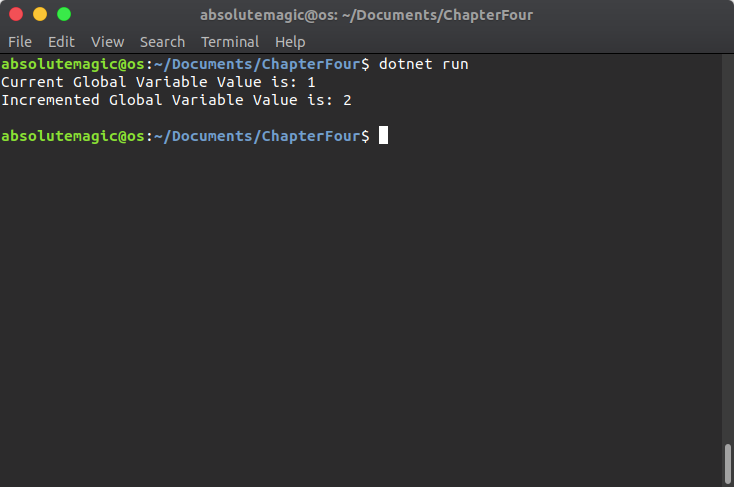
\includegraphics[width=\textwidth]{ChapterFourConsole}

As you can tell, the amount of time saved in writing the binding for native library compared to both DllImport and the Delegate Approach are very significant. You simply only have to write an interface to the native library and that eliminates the need for writing DllImport attribute repeatingly and you can also access the global variable via properties.

\chapter{Marshaling between C\# and C}
For this chapter, you'll need to create a ChapterFive directory and initialize a Dotnet Console project and to reference ''AdvancedDLSupport'' from nuget.

\section{Struct Layout}
The Layout in Struct is by default set to Sequential and you cannot use Auto layout for marshaling between Managed and Unmanaged code. Explicit Layout allows the you to explicitly define the field offsets in struct layout. This is also what enables you to  create a union in struct.

\lstinputlisting[style=customcs]{codes/Chap5/Chap5Snippet1.cs}

You may have noticed that the Val1 occupied 2 byte slots in the struct rather than Val2 being placed immediately after Val1. This is due to data alignment.  More information on that can be found here: https://software.intel.com/en-us/articles/data-alignment-when-migrating-to-64-bit-intel-architecture

To quote from that link:

\begin{coloredbox}
	The fundamental rule of data alignment is that the safest (and most widely supported) approach relies on what Intel terms "the natural boundaries." Those are the ones that occur when you round up the size of a data item to the next largest size of two, four, eight or 16 bytes. For example, a 10-byte float should be aligned on a 16-byte address, whereas 64-bit integers should be aligned to an eight-byte address. Because this is a 64-bit architecture, pointer sizes are all eight bytes wide, and so they too should align on eight-byte boundaries. - Intel 2018
\end{coloredbox}

The size of the struct shown above is 12 bytes rather than 8 bytes, because of the sequential layout rule was followed. However if you wish to override the behavior on data alignment, you can use Explicit Layout as shown below:
\newpage
\lstinputlisting[style=customcs]{codes/Chap5/Chap5Snippet2.cs}

In this struct, the size would become 8 bytes, because there is no padding required for any dangling member to fits in alignment.
\section{Pointer Marshaling}

\section{Function Marshaling}


\chapter{Marshaling between C\# and C Part 2}
\section{String Marshaling}
For this part, we'll need to create a dotnet core console project for Chapter 6 and make sure to reference ''AdvancedDLSupport'' on nuget. You will need to add a build task for this project to compile C code after building C\# code. Your CSProj file should have the following:
\lstinputlisting[style=customxml, language=XML]{codes/Chap6/Chap6Snippet1.xml}

And for this lesson, we will have a few functions to play with for string manipulation from C Library:

\lstinputlisting[style=customc, language=C]{codes/Chap6/Chap6Snippet2.c}

\section{Pointer Marshaling}

\section{Function Marshaling}
\chapter{Introduction to Common Intermediate Language}
\section{CIL Fundamentals}
The way CIL code get written are arranged by stack. So assume we have the following code in C\#:
\lstinputlisting[style=customcs]{codes/Chap7/Chap7Snippet1.cs}
That code would be compiled as follow:
\lstinputlisting[style=customcs]{codes/Chap7/Chap7Snippet2.cs}

There are few things happening here:
The shorthand CIL opcode, "ldarg.0", loads the first parameter, int a, to the stack. "ldarg.0" is a short hand opcode that you do not have to specify an argument for which parameter to load after opcode, so it save space and serves as a shortcut for runtime to infers what operation to build for that opcode.

Then "ldarg.1" do a similar operation to the above, but load the second parameter onto the stack. The "add" operation requires no arguments, but it pop off 2 items off the stack, so in "add" opcode point of view, when it pop the stack, it would see "ldarg.1" first and then "ldarg.0" second, this is something to keep in mind if you were to plan on writing a new runtime. The "add" opcode will arrange the items that were popped off the stack and do an addition operation from there (it uses the left-hand value type for addition) and then push the result of the addition to the stack.

Now that we have one remaining item in our stack, the "ret" opcode will pop the item off the stack and return that value for function return value.
\newpage
In an effort to help you actually be able to visualize and understand how this works:

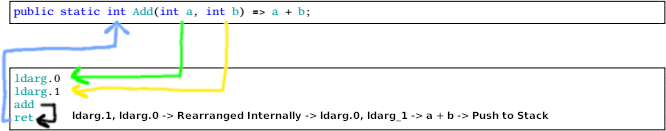
\includegraphics[width=\textwidth]{ChapSevenVisual}

There is another thing to note about CIL, the local variables have to be declared and defined before body of CIL code can be written.

\section{Special Note about the Stack}
\textit{Note: This is a simple warning for those who use Stack in .Net Framework.}

Stack is a Last In First Out, LIFO, so basically the last item you \textbf{push} to the stack is going to be the first item you get when you \textbf{pop} the stack. In .Net Framework, when you attempt to use the IEnumerator of Stack<T>, it will use the pop order in the way you read, so if you for an example have the following code:

\lstinputlisting[style=customcs]{codes/Chap7/Chap7Snippet3.cs}

There is a few things happening here, the stack would be reversed when the following code get called:

\lstinputlisting[style=customcs]{codes/Chap7/Chap7Snippet5.cs}

The stack already get reversed, because remember, the IEnumerator in Stack<T> is read by pop order, so when you pop and push to alternative stack, it rearrange the items like so:

ABC -> CBA -> ABC

To avoid this, you simply just have the following code instead of having to do any additional operations:

\lstinputlisting[style=customcs]{codes/Chap7/Chap7Snippet4.cs}

\newpage
\section{Static vs Class Member Methods}
In CIL, there is a special rule to follow for Static Method and Class Member Methods, static load the first parameter using "ldarg.0", but in class member method, it would load first parameter using "ldarg.1", not "ldarg.0". Because in class member method, "this" is a hidden parameter that get loaded when "ldarg.0" get called and this is a part of a calling convention in C\#.

\lstinputlisting[style=customcs]{codes/Chap7/Chap7Snippet6.cs}

\newpage

\section{Introducing the Dynamic Method}
For creating and building CIL code at runtime, there are three common approaches to this:
\begin{enumerate}
\item DynamicMethod
\item MethodBuilder
\item Assembly Loading via Reflection
\end{enumerate}

Although there are technically infinite amount of approaches you can do it which can involve breaking the Runtime, using unsafe code, or creating your own compiler that works similarly to Roslyn compiler infrastructure.

\subsection{Dynamic Method Approach}
A dynamic method can be defined by using the constructor and specifying the name of method, the return type and parameter types.

\lstinputlisting[style=customcs]{codes/Chap7/Chap7Snippet7.cs}

The DynamicMethod is a shortcut that uses pre-defined dynamic assembly and nest the delegate as a Global Method which are methods that are defined globally in assembly without needing to reside in a type.

\newpage

\subsection{Method Builder Approach}
A dynamic method can also be defined by first defining a dynamic assembly, module, and a type under it. It offers an additional amount of control how you emit your code by managing where code should resides in. You can also optionally choose to define method as a global method similarly to Dynamic Method above.

\lstinputlisting[style=customcs]{codes/Chap7/Chap7Snippet8.cs}

There are a number of objects that have to be defined and it chain all the way to the top starting with an Assembly, the module, the type to contains our method and finally the method itself. There are few things to explain on MethodAttributes and TypeAttributes here, similarly to C\#, we have to define our methods and types with visibility modifiers and constraints. For a static class, it's usually defined by a combination of TypeAttributes.Class, TypeAttributes.Sealed, and TypeAttributes.Abstract which essentially informs the CLR that it's a type that can't be instanced since it's sealed which cannot be inherited from and that it's an abstract which means it doesn't have a constructor to begin with. It's in all essence, a static class.

\newpage

\subsection{Assembly Loading via Reflection}
In an exceptional cases, you may have a custom compiler that generates a custom assembly library, this is one form of an unorthodox dynamic code emitting at runtime. One such form can be done through Roslyn compiler infrastructure which allows you to compile C\# snippet into a .Net assembly which can then be loaded dynamically.

\lstinputlisting[style=customcs]{codes/Chap7/Chap7Snippet9.cs}

The above constructs a .Net Assembly by leveraging Roslyn, we starts by defining our System library for .Net Assembly to reference on (so Runtime objects can be defined.) Then we have a simple snippet for C\# code to compile by using CSharpSyntaxTree that simply deconstruct our parsed text into SyntaxTree which we can then pass to CSharpCompilation object to emit the compiled code as a new .Net Assembly. Through reflection, we can then load the newly created .Net Assembly and select our Math type and it's method to call Add function.

\newpage

\section{Branches in CIL}

The CIL arrangement for branching works by specifying which "line" of CIL code to jump to or if talking about marked labels in System.Reflection.Emits, then it would jump to specified marked label. We can begin a demonstration of this by dynamically emitting a simple for loop code:

In a normal C\# snippet for a For-Loop, it can be written like this:

\lstinputlisting[style=customcs]{codes/Chap7/Chap7Snippet12.cs}

Now the same representation for above in CIL can be written as this:

\lstinputlisting[style=customcs]{codes/Chap7/Chap7Snippet10.cs}

And to help visualize what's happening here, the snippet below is a C\# equivalence to the CIL representation above:

\lstinputlisting[style=customcs]{codes/Chap7/Chap7Snippet11.cs}

\newpage

There are a number of things happening in the snippet above and it can be broken down into these steps:

\begin{enumerate}
\item Define our local variable, an index
\item Define our marks, a body and a condition
\item Emit br to condition label since for-loop requires condition to be evaluated first
\item Mark the label body at this point
\item Emit invocation for Console.WriteLine with our index variable for argument
\item Increment the index variable by 1 at the end of body stub
\item Mark label condition at this point
\item Emit Ldloc\_0 (our local variable is defined first) and Ldc\_I4 with an argument of 10
\item Emit the CLT (Compare Less Than) comparison opcode to compare index to 10
\item Emit brtrue with body label as an argument, return to body if above condition return true
\end{enumerate}

\section{OpCodes references}
You will often find a huge variety of OpCodes, but you might be asking how would you find out what each OpCode do.

The common method is to use documentation which is well maintained: \href{https://docs.microsoft.com/en-us/dotnet/api/system.reflection.emit.opcodes}{https:\/\/docs.microsoft.com\/en-us\/dotnet\/api\/system.reflection.emit.opcodes}

 For each OpCode page, it would list the description, the stack transitional behavior and the relevant overload for emit. To understand the stack transition behavior, hypothetically, you're reading on Add opcode, it would list the following Stack Transitional Behavior:

\begin{enumerate}
\item value1 is pushed onto the stack. 
\item value2 is pushed onto the stack. 
\item value2 and value1 are popped from the stack; value1 is added to value2. 
\item The result is pushed onto the stack. 
\end{enumerate}

It should be fairly clear what's happening, but if you attempt to read the same for subtraction opcode, then it would be important to know which value is a left hand value and which is the right hand value. The third item will explains that "value1 is added to value2" and that clearly define which value is left hand and vice versa.

\subsection{Note about Strict Emit Utility}
\href{https://github.com/Firwood-Software/StrictEmit}{Strict Emit} is also a free library provided by Firwood Organization  that offers a large set of extension methods for ILGenerator to further simplify and document your code.

\newpage

\section{Try Catch Finally Stubs}
The try/catch/finally in CIL are particularly similar to C\# counterpart, but there are some key differences:

\begin{enumerate}
\item There is no "Try" clause in CIL emitting, it's simply Begin/End Exception Block that enclose entire Try/Catch/Finally clauses.
\item Nested Exception Handling will have Catch/Fault blocks filter exception based on the current nested exception block.
\end{enumerate}

In the following example, the code will attempts to create a scenario that the Overflow Exception by attempting to increment an integer that have been signed to maximum value possible.

\lstinputlisting[style=customcs]{codes/Chap7/Chap7Snippet13.cs}

The way BeginCatchBlock works is that when the specified exception were caught, it would have exception available on the stack that you can pop or store into local variable, in this example, it get stored into the second local variable and then it get loaded to print to standard output.

BeginFinallyBlock except a stub of code that will happen in either cases when exception is thrown and when code run successfully without exception.
\chapter{Advanced CIL Programming}
\section{Constructing a Type at Runtime}
One of the more advanced use of Runtime code emitting involves the use 
\backmatter
% bibliography, glossary and index would go here.

\end{document}